%  CONCLUSION au lieu de extension 

%% maybe add extension as a part of the conclusion for this chapter 
\section{Benchmarking protocol to extend reproducibility}\label{sec:bench_extension}

We propose to extend the benchmarking framework suggested by the \emph{Collaboratory on Experimental Evaluation of Software and Systems in Computer Science}\footnote{\url{http://evaluate.inf.usi.ch/}} to address those limitations.
Instead of only presenting the four primary aspects of their guidelines that were mentioned previously in section ~\ref{sec:benchmarking_reproducibility}, we propose an abstract model to describe an empirical experiment:

\emph{context}: the hardware and the software configuration for the actual experiment, the purpose of this part is to provide extra information to help readers have a better judgement on the results and to be able reproduce the experiment while diminishing the impact of the external factor .
An \emph{orchestrator} which its job to run the experiment.
The orchestrator provides three interfaces:

\emph{Workload interface}: provides a set of functions that should be implemented by the workload  and called by the each candidate in the experiment.
Observer interface: provides a set of metrics that are collected by the orchestrator during the expermentation. note that some of those metrics are external, such the energy consumption of the system , execution time, execution stack ..etc .
\begin{figure}[!htb]
    \center{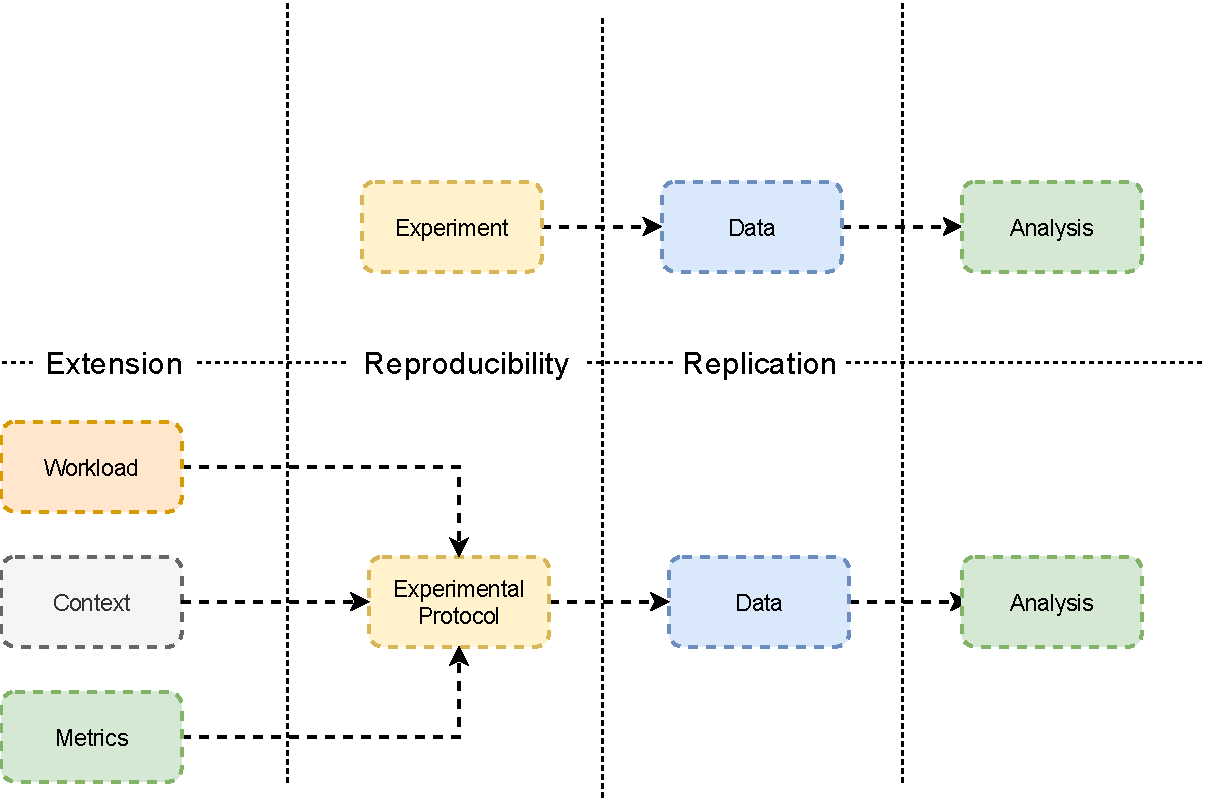
\includegraphics[width=\linewidth]{imgs/benchmarkingprotocol}}
    \caption{Benchmarking protocol}\label{fig:benchmarkingprotocol}
\end{figure}
Figure~\ref{fig:benchmarkingprotocol} explains in detail the relationship within each component of the protocol.
First of all, we should start with the orchestrator which is the kernel of the experiment. Most of the time this kernel should represent the constants parts of the experiment.
The orchestrator is responsible for the following  for the coordination between the workload and the candidate, therefore it provides an interface that is implemented by each workload.
Later this interface will be provided to each candidate by the orchestrator. Like this we will remove any bias of dependency between the workload and the candidates, which will alow us to extend both parts without any change in the code.
Instead of retrieving the data directly from the experiment, we suggest to use an observator to allow the extension of the metrics, this observer in general should be outside the experiment to be able to gather as many informations without impacting the the code.


By the end of this study, we have gathered enough guidelines to make the tests more reproducible, accurate and extensible.
We created a set of new tests named \textbf{energy tests} which are more similar to performance tests.
Thanks to the work of two interns [Mamadou and Adrien] we created a CI/CD platform to measure the energy consumption of Java projects and we could track the evolution of the this energy across different stages of the project.
In the figure below we see an example of this plugin.
For more details please visit the gitlab repository\footnote{\url{https://gitlab.inria.fr/mamdiall/J-Joules}}~\footnote{\url{https://gitlab.inria.fr/mamdiall/jjoules-plugin}} .

% \begin{figure}%[!htb]
%     \center{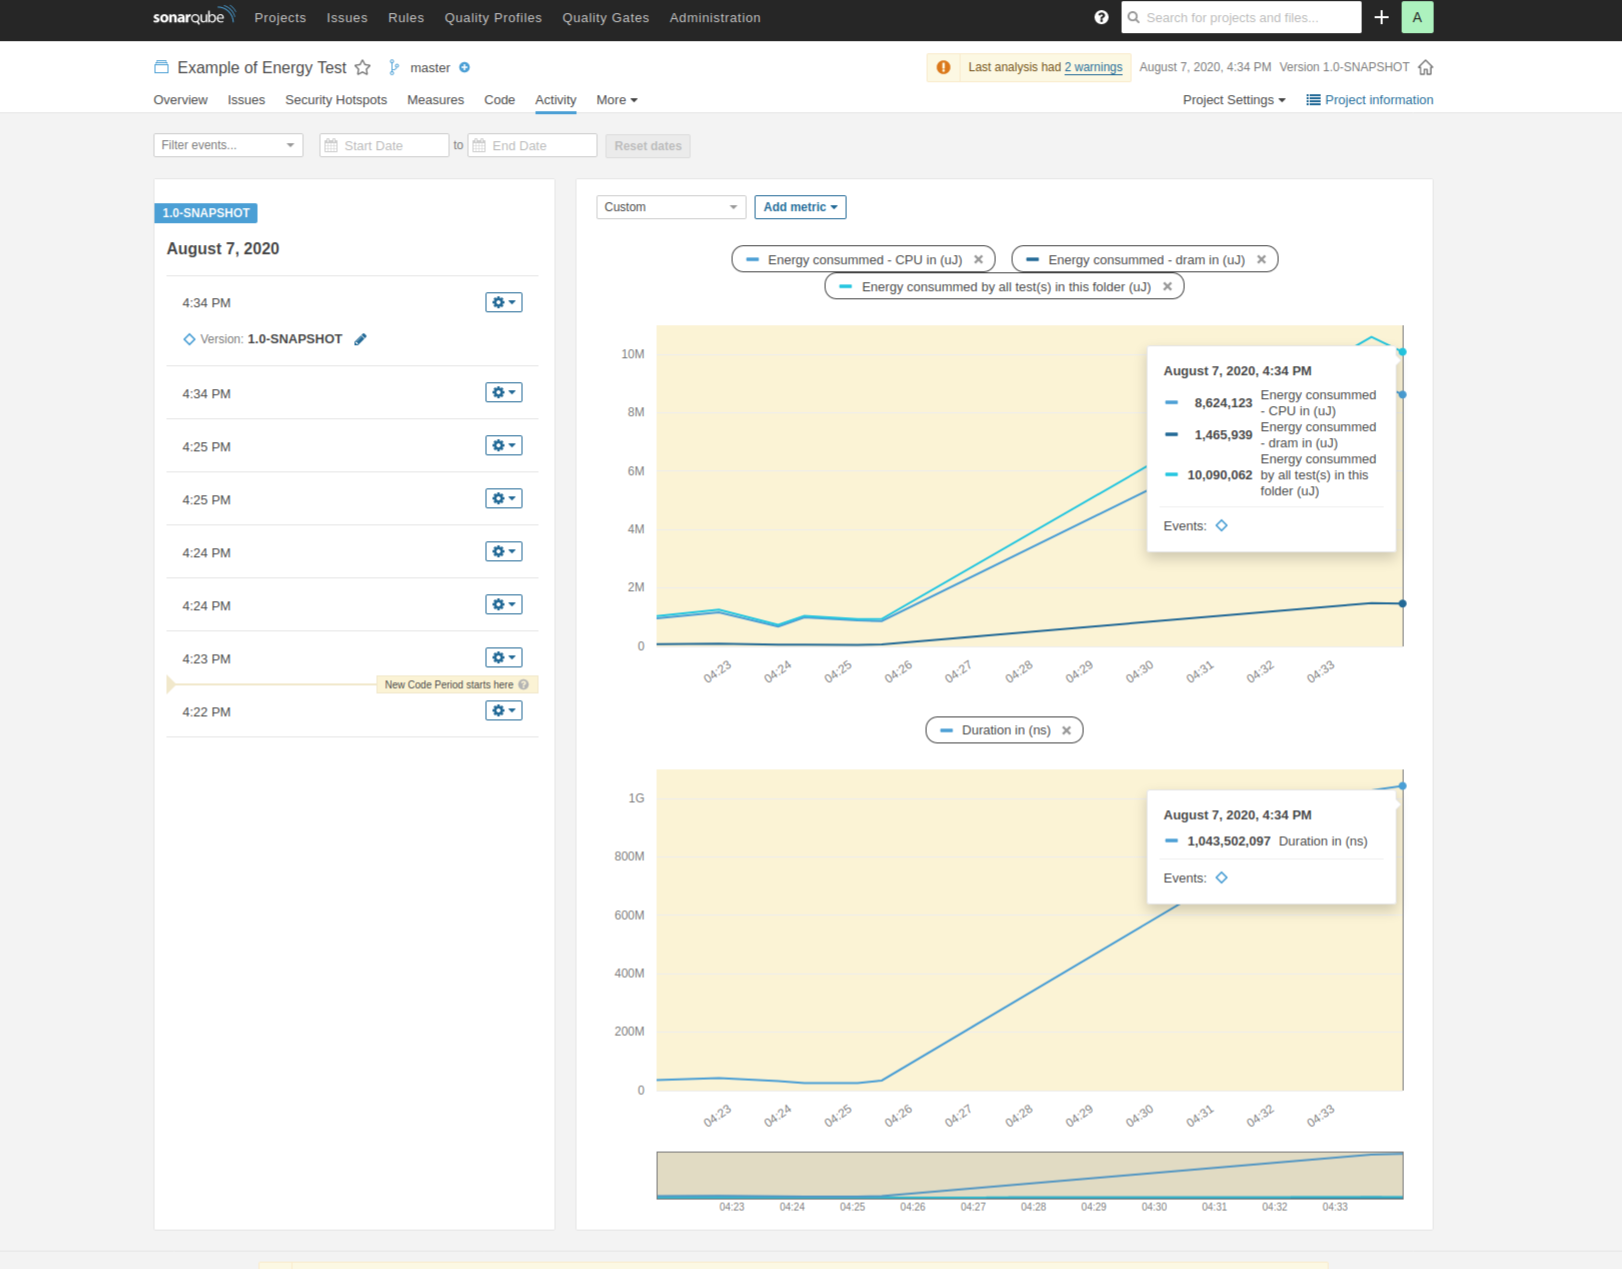
\includegraphics[width=.9\linewidth]{imgs/JunitSonarplugin}}
%     \caption{Example of the Junit Sonar Plugin}\label{fig:sonar_plugin}
% \end{figure}
\section{Conclusion \note{missing}}